\documentclass[12pt, a4paper]{article}
\usepackage[a4paper, includeheadfoot, mag=1000, left=2cm, right=1.5cm, top=1.5cm, bottom=1.5cm, headsep=0.8cm, footskip=0.8cm]{geometry}
% Fonts
\usepackage{fontspec, unicode-math}
\setmainfont[Ligatures=TeX]{CMU Serif}
\setmonofont{CMU Typewriter Text}
\usepackage[english, russian]{babel}
% Indent first paragraph
\usepackage{indentfirst}
\setlength{\parskip}{5pt}
% Diagrams
\usepackage{graphicx}
\usepackage{float}
% Page headings
\usepackage{fancyhdr}
\pagestyle{fancy}
\renewcommand{\headrulewidth}{0pt}
\setlength{\headheight}{16pt}
%\newfontfamily\namefont[Scale=1.2]{Gloria Hallelujah}
\fancyhead{}

\usepackage{amsmath}

\graphicspath{ {images/} }

\usepackage{listings}
\lstdefinestyle{lablisting}{
  basicstyle=\scriptsize\ttfamily,
  numbers=left,
  stepnumber=1,
  otherkeywords={EOF, O\_RDONLY, STDIN\_FILENO, STDOUT\_FILENO, STDERR\_FILENO},
  numbersep=10pt,
  showspaces=false,
  showstringspaces=false
}

\newcommand{\specialcell}[2][l]{%
  \begin{tabular}[#1]{@{}l@{}}#2\end{tabular}}

\begin{document}

% Title page
\begin{titlepage}
\begin{center}

\textsc{Национальный исследовательский университет ИТМО\\[4mm]
Факультет программной инженерии и компьютерной техники}
\vfill
\textbf{Практическое задание №1\\[4mm]
по дисципение Теория Автоматов\\[4mm]
Взаимная транспозиция автоматов Мили и Мура\\[4mm]
}
\textit{Вариант 11\\[16mm]}
\begin{flushright}
Студент: Саржевский Иван
\\[2mm]Группа: P3302
\\[2mm]Преподаватель: Тропченко Александр Ювенальевич
\end{flushright}
\vfill
г. Санкт-Петербург\\[2mm]
2020 г.

\end{center}
\end{titlepage}

\section*{Цель}

Практическое освоение методов взаимного преобразования автоматных моделей
Мили и Мура. Проверка абстрактных автоматов Мили и Мура на эквивалентность.

\section*{Задание}

Исходный абстрактный автомат задан графическим способом. При переходе от
автомата Мура (A) к автомату Мили (B):
$$S_A = (A_A, Z_A, W_A, \delta_A, \lambda_A, a_{1A}) \to S_B = (A_B, Z_B, W_B, \delta_B, \lambda_B, a_{1B})$$
и наоборот:
$$S_B = (A_B, Z_B, W_B, \delta_B, \lambda_B, a_{1B}) \to S_A = (A_A, Z_A, W_A, \delta_A, \lambda_A, a_{1A})$$

При этом их входные и выходные алфавиты должны совпадать:
$$Z_A = Z_B; W_A = W_B$$

\section*{Исходные данные}

Вариант 11.

\begin{center}
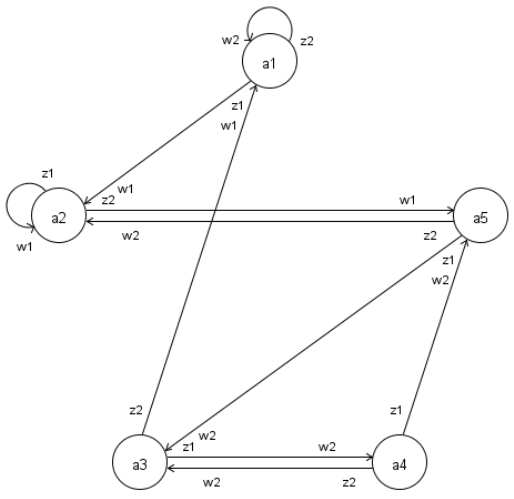
\includegraphics[scale=2.0]{input-graph}\\
\end{center}

\noindent $S_B = (A_B, Z_B, W_B, \delta_B, \lambda_B, a_{1B})$\\
$A_B = \{a_1, a_2, a_3, a_4, a_5\}$\\
$Z_B = \{z_1, z_2\}$\\
$W_B = \{w_1, w_2\}$\\

\section*{Переход от автомата Мили к автомату Мура}

\subsection*{Определим множества A}

\noindent $A_1 = \{a_1W_1, a_1W_2\}$\\
$A_2 = \{a_2W_1, a_2W_2\}$\\
$A_3 = \{a_3W_2\}$\\
$A_4 = \{a_4W_2\}$\\
$A_5 = \{a_5W_1, a_5W_2\}$

\subsection*{Присвоим b}

\noindent $A_1 : \begin{cases}
  a_1W_1 = b_1 \\
  a_2W_2 = b_2
\end{cases}$\\
$A_2 : \begin{cases}
  a_2W_1 = b_3 \\
  a_2W_2 = b_4
\end{cases}$\\
$A_3 : \; \; \: \, a_3W_2 = b_5$\\    % me and the boys when the
$A_4 : \; \; \: \, a_4W_2 = b_6$\\    % align* centers equation:\
$A_5 : \begin{cases}
  a_5W_1 = b_7 \\
  a_5W_2 = b_8
\end{cases}$\\

\subsection*{Полученный автомат Мура}

\begin{center}
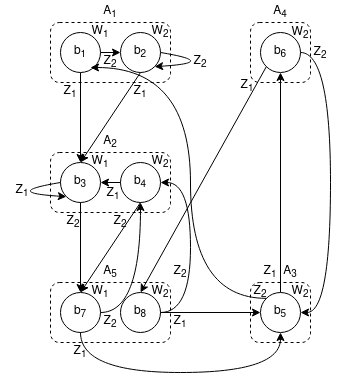
\includegraphics[scale=0.8]{moore}\\
\end{center}

\subsection*{Проверка автоматов на эквивалентность}

Проверим, что реакции исходного и полученного автомата на одинаковое входное
слово совпадают. В качестве проверочного слова была выбрана посдедовательность
сигналов \texttt{$z_1 z_2 z_1 z_1 z_1 z_2 z_1 z_2 z_1 z_1 z_2 z_2 z_2$}, так
как при такой посдедовательности осуществляются все возможные переходы в
исходном графе.

\noindent
\begin{small}
\begin{tabular}{ l | l }
  \normalsize{Автомат Мили} & \normalsize{Автомат Мура} \\
  \texttt{z1 z2 z1 z1 z1 z2 z1 z2 z1 z1 z2 z2 z2} & 
    \texttt{z1 z2 z1 z1 z1 z2 z1 z2 z1 z1 z2 z2 z2} \\
  \texttt{a1 a2 a5 a3 a4 a5 a2 a2 a5 a3 a4 a3 a1 a1} &
    \texttt{b1 b3 b7 b5 b6 b8 b4 b3 b7 b5 b6 b5 b1 b2} \\
  \texttt{w1 w1 w2 w2 w2 w2 w1 w1 w2 w2 w2 w1 w2} &
    \texttt{\_\_ w1 w1 w2 w2 w2 w2 w1 w1 w2 w2 w2 w1 w2}
\end{tabular}
\end{small}

Можно сделать вывод, что реакция автоматов на одинаковое входное слово
эквивалентна, за исключением того, что реакция автомата Мура сдвинута на один
такт. Это объясняется тем, что реакция на входной сигнал у этого автомата
наступает только в следующем такте. Результат свидетельствует об эквивалентности
автоматов.

\section*{Переход от автомата Мура к автомату Мили}

При переходе от автомата Мура к автомату Мили алфавиты состояний совпадают,
т.е. $A_A = A_B$. Функции переходов тоже совпадают, а для определения функции
выходов выходные сигналы с вершин опускаются на входные дуги.

\subsection*{Полученный автомат Мили}

\begin{center}
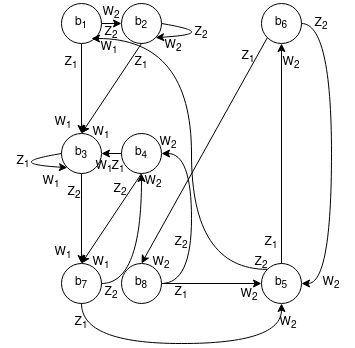
\includegraphics[scale=0.8]{mili}\\
\end{center}

\end{document}
